\section{Define}
Nachdem erste Interviews mit potentiellen Nutzern durchgeführt wurden und das Problem besser verstanden wurde, können nun unsere Grundannahmen aufgestellt und einem LeanUX Canvas dargestellt werden. Zudem werden Personas erfasst. Hier ist es wichtig zu Erwähnen, dass es sich nur um eine erste Iteration handelt und sich die Grundannahmen und Hypothesen sicherlich weiterentwickeln bzw. ändern werden.

\subsection{Erstellen eines Lean UX Canvas} \label{lean_ux_canvas}
Abbildung \ref{lean_ux_canvas_image} zeigt den aufgestellten LeanUX Canvas in der 1. Iteration. Der Canvas beschreibt unsere ersten Annahmen und Lösungsvorschläge, kann jedoch noch in vielen Iterationen überarbeitet werden. Die 1. Iteration wurde nach den ersten Interviews mit potentiellen Nutzern durchgeführt.
Folgend werden unsere Erfahrungen und Probleme beim Erstellen des Canvas genauer erläutert:

\begin{enumerate}
    \item \textbf{Business Problem}: Die Identifikation der Probleme stellte sich relativ leicht heraus. Beim Erstellen des Fragebogens haben wir uns stark auf die Identifikation der zugrundeliegenden Probleme konzentriert. Eine Technik, die uns hier sehr geholfen hatte, ist die sogenannte ``5. Why-Methode''\footnote{https://medium.com/productmanagement101/learn-about-the-five-whys-technique-78283d75800f}. Die Probleme mussten nur noch aus dem Interview zusammengefasst werden.
    \item \textbf{Business Outcomes}: Das Finden von konkreten Metriken zum Messen der Problemlösung stellte sich nun bereits schwieriger dar. Wir haben einerseits rein quantitative Metriken aufgestellt, welche wir anhand von Zahlen messen können, andererseits aber auch qualitative Metriken aufgestellt. Die qualitativen Metriken sind insbesondere am Anfang sehr wichtig, da man oft noch nicht genug Daten sammeln kann, um statistisch signifikante Resultate erhalten zu können. Die qualitativen Metriken werden mithilfe von Kurzinterviews oder Fragebogen erfasst. \citep{croll2013lean}
    \item \textbf{Users}: Das Finden der wichtigsten Usergruppe war relativ einfach, da wir eine klar definierte Gruppe von Leute bereits definiert haben. Neu war die Überlegung, dass es am Anfang vor allem Sinn machen würde, wenn wir die Nutzer gerade Gruppenweise auf unsere Lösung bringen können. Dadurch können sich die Nutzer bereits innerhalb der Gruppen organisieren.
    \item \textbf{User Outcomes and Benefits}: Dieser Teil hat uns besonders geholfen zu überlegen, auf welche Bereiche unsere Lösung besonders fokussieren soll. Dieser Bereich konnten wir für die anschliessende Lösungsfindung als eine Art ``Checkliste'' verwenden, um zu kontrollieren ob die anschliessende Lösung die Punkte deckt.
    \item \textbf{Solutions}: Die Lösungsfindung war wahrscheinlich bereits etwas vor den anderen Bereichen erfolgt. Die Lösung hatten wir bereits schon in der Problemanalyse im Kopf. Wir denken jedoch, dass es relativ viel Zeit braucht, bis man sich wirklich an dieses Mindset vom problemorientierten Design Thinking gewöhnt hat. Die ganzen Analysen aus der Empathize Phase konnten uns jedoch sehr gut helfen, auf welche Bereiche wir uns besonders fokussieren sollen.
    \item \textbf{Hypotheses}: Aufgrund der aufgestellten Lösung konnten nun Hypothesen aufgestellt werden, welche letztendlich das zugrundeliegende Problem mit der Lösung verbinden sollen. Wir empfinden diesen Schritt als wichtigster Schritt im ganzen Canvas, da man nun alle Elemente zusammen bringt.
    \item \textbf{Risks}: In diesem Bereich soll die Hauptursache formuliert werden, warum unsere Lösung scheitern könnte. Dies war für uns relativ schnell klar, da es sich bei der Lösung um ein Produkt handelt, das stark abhängig von den Nutzern und vor allem auch von der Aktivität der Nutzer auf der Plattform lebt. Ein Beispiel von neuen Applikationen, welche wahrscheinlich zum grössten Teil an diesem Grund scheitern sind neue soziale Medien wie bspw. Vero. \footnote{https://www.thenational.ae/arts-culture/comment/the-rise-and-fall-of-social-media-app-vero-1.709839}.
    \item \textbf{Next Steps}: Dieser Schritt lässt sich sehr einfach anhand des Vorgehensmodells nach Design Thinking realisieren.
\end{enumerate}

\newgeometry{a4paper,left=1in,right=1in,top=1in,bottom=1in,nohead}
\begin{landscape}
    \begin{figure}[H] 
        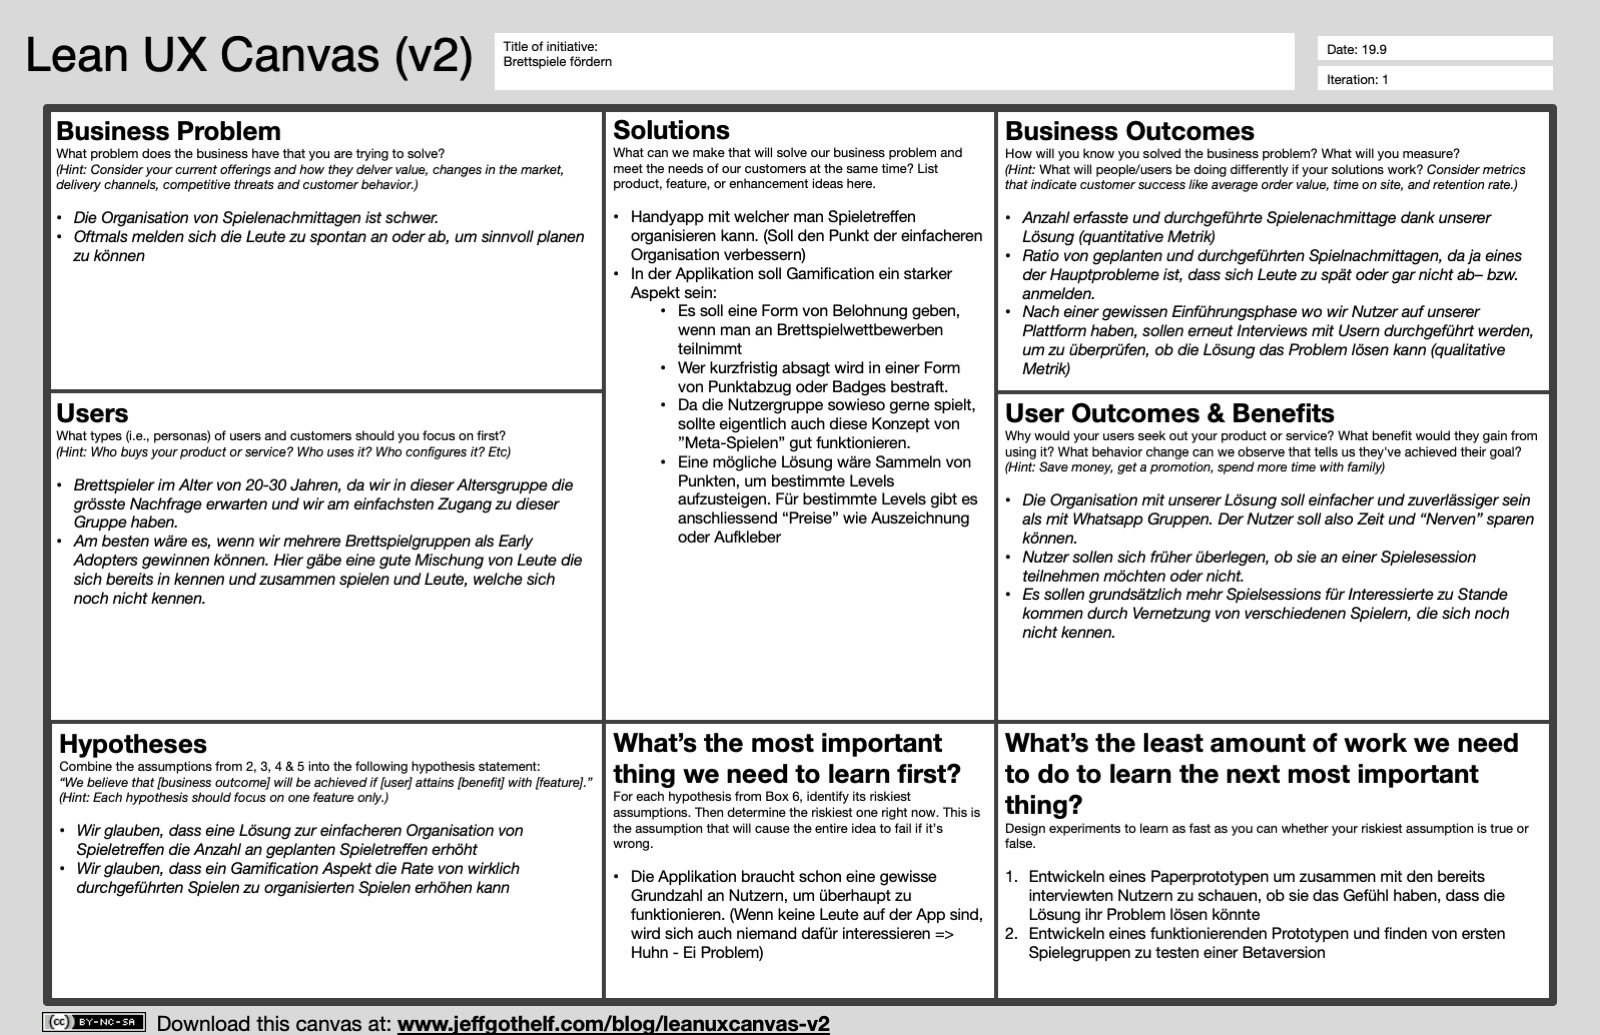
\includegraphics[width=24cm]{images/LeanUXCanvas.jpg}
        \caption{LeanUX Canvas}
        \label{lean_ux_canvas_image}  
    \end{figure}
\end{landscape}
\restoregeometry 

\subsection{Entscheid über die Art der Lösung}
Da wir uns nun schon mit dem Fachbereich bekannt gemacht haben, geht es nun darum, zu Entscheiden, in welcher Form die Lösung implementiert werden soll. Konkret kamen uns die Formen mobile Webseite oder App in den Sinn, da das Organisieren von Spielsessions oftmals sehr kurzfristig geschieht und schnell gehen muss, wodurch sich ein Smartphone bestens eignet. Mit dem Smartphone kann man fast überall und jederzeit eine neue Spielsession erstellen, oder auf eine Einladung reagieren. Da für Einladungen zu Sessions Benachrichtigungen verwendet werden, eignet sich eine 
App besser, da damit auch Benachrichtigungen versendet werden können. Moderne Browser, wie Chrome, unterstützen zwar auch Benachrichtigungen, jedoch verlangen diese die Zustimmung des Benutzers und es ist nicht sicher, ob die Benachrichtigungen dann auch mit allen Browsern funktionieren würden. Im Interview hat sich auch gezeigt, dass Samuel Müller kein Fan von mobilen Webseiten ist.

\subsection{Personas}
Um das Produkt kundenorientiert entwickeln zu können, muss man wissen, wer die Kunden sind und welche Bedürfnisse die Kunden haben. Man muss sich in die Kunden einfühlen können. Um dies einfacher zu erreichen, werden in kundenorientierten Produktentwicklungsprozessen sogenannte Personas entworfen und zur Hilfe gezogen.
\subsubsection{Kurze Theorie über Personas}
'Eine Persona ist die Verkörperung des Problems, Bedürfnisses, Ziels und Verhaltens einer hypothetischen Kunden- oder Nutzergruppe. Personas basieren auf relevanten Informationen und Einsichten der Ersteller. Sie sind im Grunde genommen eine Sammlung von Annahmen, die  im Verlauf des Kunenentwicklungsprozesses getestet und verfeinert werden müssen. [...] Personas werden genutzt, um Empathie mit den Problemen unserer Zielgruppen zu erzeugen und um die Diskussion von unsernen individuellen Präferenzen wegzubewegen und hin zu dem, was die gewählte Persona als wertvoll erachten würde - dem zu erledigenden Job.' \cite{humble2017lean}
\subsubsection{Vorgehen}
Um eine Persona zu erschaffen, die die Kunden unseres Produkts repräsentiert, sind wir folgendermassen vorgegangen:
Im FFHS-Modul ``Mensch-Computer-Kompetenzen'' durften wir schon das Konzept der Personas kennenlernen und auch schon eigene Personas für ein Projekt entwerfen. Daraus konnten wir natürlich schon die Erfahrung sammeln, dass es eine kreative Aufgabe ist und weit weg von objektiver Wissenschaft.
Des weiteren haben wir uns informiert, wie es in den Firmen, in denen wir arbeiten, gehandhabt wird. Wir haben uns Fragen gestellt, wie: Gibt es ein Customer-Experience-Management in der Unternehmung? Wenn ja, werden Methoden wie die Personas eingesetzt?

Post und PostFinance:
In beiden Unternehmungen versucht man sehr kundenorientiert zu arbeiten und Produkte erschaffen, die der Kunde/die Kundin auch will und verwendet. Es gibt ganze Teams, die spezialisiert in diesem Bereich sind und Projektteams und Fachabteilungen mit innovativen Vorgehensweisen und Workshops etc. unterstützen. Im Produktentwicklungsprozess werden in beiden Unternehmungen in Customer-Experience-Workshops User-Stories entworfen und man definiert Requirements, indem man sich bewusst in die Rolle einer Persona begibt.
Bei der PostFinance gibt es neuen Persona für Privatkunden und 7 Persona für Geschäftskunden. Damit man sich ein gutes Bild über die Persona machen kann, besitzt jede Persona einen Steckbrief. Auf diesem Steckbrief sind branchenspezifische Angaben drauf (z.B. Digitalisierungsgrad, Kreditkartenbesitzer etc.), aber auch Hobbies etc, um mit der Persona Empathie aufbauen zu können. Zwei der PostFinance-Privatkunden-Personas stehen sogar als lebendgrosse Kartonfigur im Hauptsitz!


Die Persona Remo, die wir für unser Projekt entworfen haben, stützt sich auf die Idee der PostFinance, einen übersichtlichen Steckbrief zu erfassen. Die Bilder sollen den Prozess unterstützen, damit man sich gut in die Person versetzen kann.
\subsubsection{Persona Remo}
Remo's Vorbild ist ein Kollege eines Projektmitgliedes, das gerne Gesellschaftsspiele spielt und Spieleabende organisiert. Die Persona soll jung und dynamisch sein und auch das gewisse 'Etwas' haben, damit man Sympathie zu ihr aufbauen kann. Zum Beispie: Der Studentenjob in der Gelateria di Berna gibt der Persona etwas Persönliches, Lokales. Man verbindet mit der Gelateria di Berna vielleicht selber Emotionen und kann sich so eher ein Bild von der Persona ausmalen.
Ideen für gewisse Ausprägungen der Persona stammen aus dem Alltag und wurden kreativ auf dem A4-formatigen Steckbrief dargestellt nach dem Vorbild der PF-Persona-Steckbriefe.
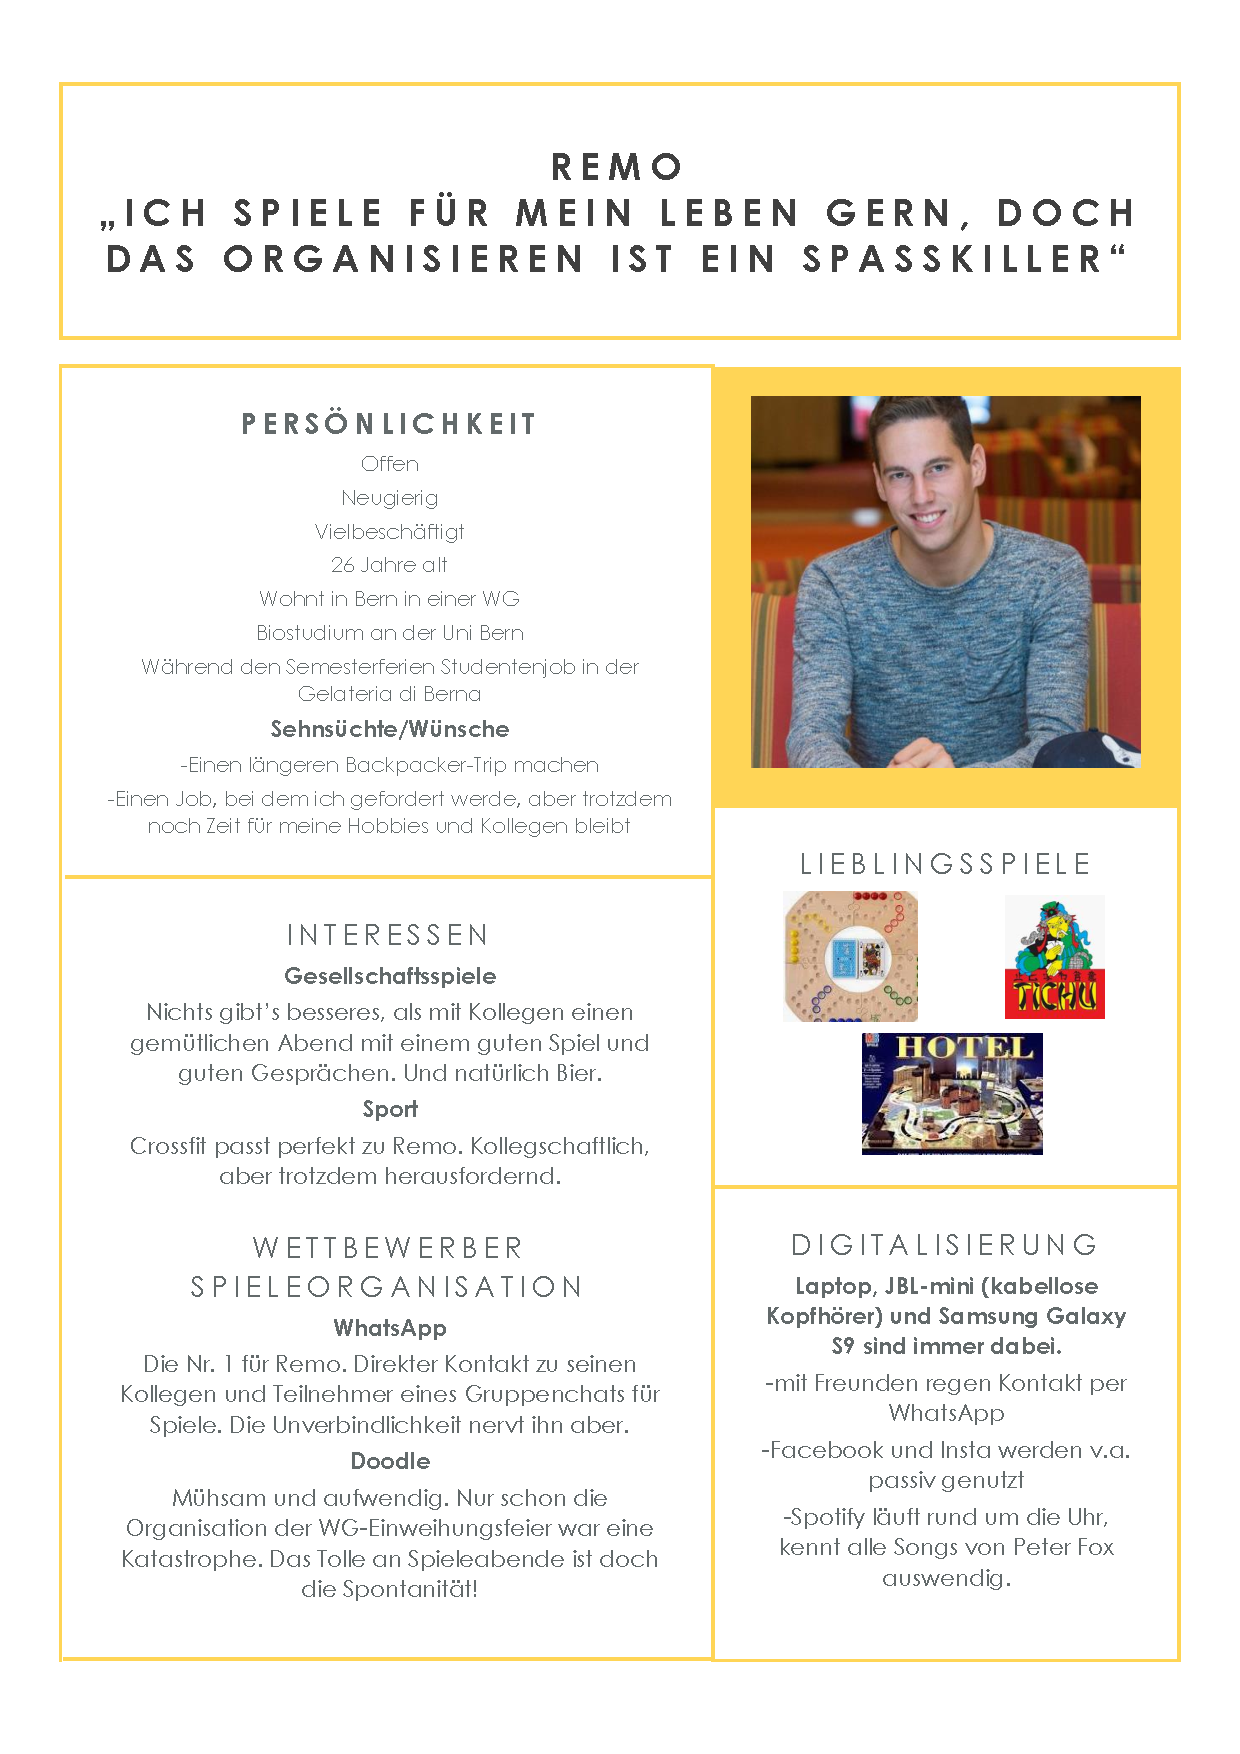
\includepdf[frame=true]{images/Persona_Remo.pdf}
\subsubsection{Nutzung der Persona}
Die Persona Remo soll natürlich nicht nur schön und lustig sein, sondern auch eingesetzt werden. In unserem Anforderungsmanagement spielt die Persona eine grosse Rolle. Bei jeder Anforderung überlegten wir, was Remo wohl dazu sagen würde und welches Bedürfnis noch nicht durch die Anforderung abgedeckt wurde. 
\newpage
\subsection{Anforderungen}
\subsubsection{Theorie der Userstories}
Die Persona Remo sowie die Stakeholder haben Bedürfnisse an das neue Produkt. Um 'lean' zu bleiben und nicht zu viel Zeit in eine unnötig lange und unspezifische Anforderungsdokumentation zu investieren, haben wir uns entschieden, die Anforderungen als User-Stories zu definieren. Dabei werden die Bedürfnisse in Prosa verfasst. Die Persona Remo hilft uns dabei. Wir können uns in die Perspektive von Remo begeben und unsere Wünsche in der Ich-Position verfassen.
\subsubsection{Vorgehen}
Mithilfe des Interviews mit Samuel Müller wurden die Bedürfnisse eruiert und hier gesammelt. Ausserdem haben wir uns in die Persona Remo hineingedacht und uns vorgestellt, dass wir in drei Tagen einen Spieleabend organisieren würden. Die Wünsche haben wir in User-Stories dokumentiert.
\subsubsection{User-Stories}
\begin{enumerate}
\item Als Spieleorganisator Remo möchte ich eine App haben, mit der ich den Spieleabend von A bis Z organisieren kann, damit die Organisation einfacher wird.
\item Als Spieleorganisator Remo möchte ich in der App mit meinen Spielekollegen chatten können, um die Kommunikation vor, während und nach dem Spieleabend zu vereinfachen.
\item Als Spieleorganisator Remo möchte ich, dass die Teilnehmer definitiv zusagen müssen, damit der Spieleabend auch wirklich stattfinden kann.
\item Als Spieleorganisator Remo möchte ich eine Funktion haben, damit man den Ort des Spieleabends koordinieren kann, damit nicht nur ich als Organisator den Ort zur Verfügung stellen muss.
\item Als Spieleorganisator Remo möchte ich in der App mit meinen Mitspielern schon vor dem Treffen bestimmen können, welche Spiele wir spielen, damit es keine Streitereien und Diskussionen am Abend gibt und ein Wissen der Spielregeln als Voraussetzung für den Spieleabend gilt.
\item Als Spieleorganisator Remo möchte ich eine Funktion haben, dass ich einen Spieleabend 'öffentlich' machen kann, damit ich neue Spielefreunde kennenlernen kann.
\item Als Entwickler möchte ich Gamification ins Spiel einbauen, damit die Benutzer Spass haben, meine App zu verwenden und Konkurrenzprodukte langweiliger wirken.
\item Als Spieler Samuel möchte ich meine Spiele übersichtlich in der App dargestellt haben, damit ich den Überblick nicht verliere.
\item Als Spieler Samuel möchte ich aus der App auf meinen Kalender zugreifen können, um die Daten einfacher festlegen zu können und keinen Terminkonflikt zu verursachen.
\item Als Spieler Samuel möchte ich, dass die Mitspieler rasch antworten müssen (zu-/absagen), damit ich den Termin nicht umsonst blocken muss.
\item Als Spieleorganisator Samuel möchte ich definieren können, welches Fähigkeitslevel potenzielle Mitspieler bei Spielen haben müssen, damit es auch zu interessanten, herausfordernden Spielen kommt.
\item Als Spieleorganisatior Samuel möchte ich definieren können, ob die Spielesession öffentlich oder privat sein soll, damit ich nach Lust und Laune mit fremden Leuten oder nur mit Freunden spielen kann.
\end{enumerate}


